\documentclass[10pt,twocolumn,letterpaper]{article}

\usepackage[utf8]{inputenc}
\usepackage[margin=0.75in]{geometry}
\usepackage{amsmath,amssymb,amsfonts}
\usepackage{booktabs}
\usepackage{graphicx}
\usepackage{hyperref}
\usepackage{xcolor}
\usepackage{microtype}
\usepackage{cite}
\usepackage{tikz}
\usetikzlibrary{shapes.geometric, arrows.meta, positioning}

\hypersetup{
    colorlinks=true,
    linkcolor=blue!70!black,
    citecolor=blue!70!black,
    urlcolor=blue!70!black
}

\title{\textbf{Verified Attention Protocol (VAP):}\\
An Open, Evidence-Centric Infrastructure for Verifiable Human Engagement}

\author{
  \textbf{Karakana Labs} \\
  \texttt{research@karakana.io}
}

\date{\today}

\begin{document}

\maketitle

\begin{abstract}
Human attention is the primary economic engine of digital media, education, compliance, and AI evaluation, yet the modern Internet lacks an independent infrastructure layer to verify that a human has authentically engaged with digital content. Existing metrics rely on self-reported platform proxies (impressions, clicks, dwell times) vulnerable to click farms, headless automated agents, and misaligned economic incentives. In this paper, we introduce the \textbf{Verified Attention Protocol (VAP)} and its reference implementation, the \textbf{Verified Attention Engine (VAE)}. Grounded in an \emph{Evidence-Centric Architecture (ECA)}, VAP decouples observation from application logic: raw client signals are transformed into immutable, cryptographically hashed evidence, evaluated via calibrated probabilistic models, and certified through Ed25519-signed \emph{Proofs of Attention (PoA)}. We demonstrate how VAP guarantees sub-second verification, mitigates synthetic bot engagement without intrusive surveillance, and creates an open, privacy-preserving standard for digital attention economics.
\end{abstract}

\section{Introduction}
The architectural history of the Internet is characterized by the progressive institutionalization of open coordination protocols: DNS for hierarchical naming, TLS for transport confidentiality, HTTP for resource retrieval, and TCP/IP for packet routing. Each foundational capability was abstracted into a vendor-neutral primitive rather than an application-specific feature.

Despite this evolution, the Internet's scarcest cognitive and commercial resource—\textbf{human attention}—remains structurally unverified. An estimated 20\% to 40\% of global digital ad spend is squandered on automated non-human traffic, click farms, and ghost impressions. In professional education and corporate compliance, institutions depend on superficial completion flags that certify clicking rather than cognitive comprehension. Furthermore, in the training of artificial intelligence systems (specifically Reinforcement Learning from Human Feedback), synthetic data and unverified annotator inputs pollute downstream models.

Existing solutions cannot simply be retrofitted:
\begin{itemize}
    \item \textbf{Ad Networks:} Suffer from structural conflicts of interest where platforms simultaneously monetize impressions and audit their legitimacy.
    \item \textbf{Analytics Engines:} Record \emph{syntax} (that an event occurred) rather than \emph{semantics} (whether genuine human cognition was engaged).
    \item \textbf{Identity \& CAPTCHAs:} Verify identity or humanity at a discrete snapshot, offering zero guarantees regarding ongoing session engagement.
\end{itemize}

VAP provides the missing primitive: a standard, privacy-preserving, and mathematically calibrated verification protocol for human engagement.

\section{Evidence-Centric Architecture (ECA)}
VAP is founded on the immutable axiom: \emph{No decision without evidence; no evidence without provenance.} The protocol strictly mandates a non-invertible pipeline:

\begin{equation*}
\mathcal{O} \longrightarrow \mathcal{E} \longrightarrow \mathcal{C} \longrightarrow \mathcal{P}_{\text{conf}} \longrightarrow \mathcal{V} \longrightarrow \text{PoA}
\end{equation*}

\subsection{Architectural Primitives}
\begin{itemize}
    \item \textbf{Observation ($\mathcal{O}$):} Uninterpreted micro-signals captured from client runtimes (scroll velocity, micro-pauses, viewport dwell, focus transitions).
    \item \textbf{Evidence ($\mathcal{E}$):} Normalized, validated records deterministically hashed with session scope, timestamp, and client provenance. Once recorded, evidence is append-only and immutable.
    \item \textbf{Claim ($\mathcal{C}$):} Formal semantic assertions derived from evidence (e.g., $\text{claim}_{\text{reading}} \equiv \text{dwell} \ge 30\,\text{s} \land \text{engagement\_score} \ge 0.45$).
    \item \textbf{Calibrated Confidence ($\mathcal{P}_{\text{conf}}$):} A deterministic probability $p \in [0.0, 1.0]$ derived using Platt scaling or isotonic regression over verified evidence distributions.
    \item \textbf{Proof of Attention (PoA):} An unforgeable token signed by an authorized verifier certifying that session requirements met policy criteria with calibrated confidence.
\end{itemize}

\begin{figure}[htbp]
\centering
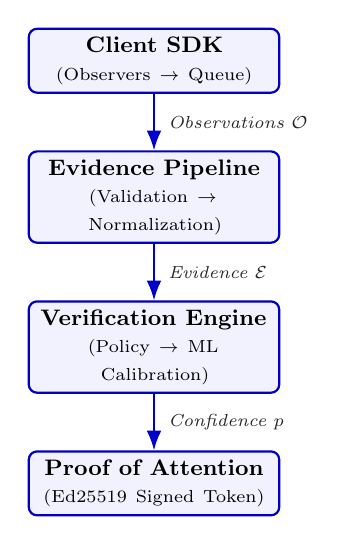
\begin{tikzpicture}[
    auto,
    scale=0.9,
    every node/.style={transform shape},
    block/.style={
        rectangle,
        draw=blue!75!black,
        thick,
        fill=blue!5,
        text width=3.3cm,
        text centered,
        rounded corners=3pt,
        minimum height=0.9cm,
        font=\small\bfseries
    },
    line/.style={
        draw=blue!80!black,
        -{Latex[length=2.5mm]},
        thick
    },
    labelnode/.style={
        font=\scriptsize\itshape,
        text=black!85,
        align=center
    }
]
    \node [block] (client) {Client SDK\\{\normalfont\scriptsize(Observers $\rightarrow$ Queue)}};
    \node [block, below=0.8cm of client] (pipeline) {Evidence Pipeline\\{\normalfont\scriptsize(Validation $\rightarrow$ Normalization)}};
    \node [block, below=0.8cm of pipeline] (verifier) {Verification Engine\\{\normalfont\scriptsize(Policy $\rightarrow$ ML Calibration)}};
    \node [block, below=0.8cm of verifier] (poa) {Proof of Attention\\{\normalfont\scriptsize(Ed25519 Signed Token)}};
    
    \path [line] (client) -- node [right=2pt, labelnode] {Observations $\mathcal{O}$} (pipeline);
    \path [line] (pipeline) -- node [right=2pt, labelnode] {Evidence $\mathcal{E}$} (verifier);
    \path [line] (verifier) -- node [right=2pt, labelnode] {Confidence $p$} (poa);
\end{tikzpicture}
\caption{The Verified Attention Protocol Verification Pipeline.}
\label{fig:pipeline}
\end{figure}

\section{Threat Model and Adversarial Defense}
VAP explicitly models adversarial attacks attempting to mint illegitimate Proofs of Attention.

\subsection{Attack Vectors}
\begin{enumerate}
    \item \textbf{Static Bot Scripts:} Headless scripts (Puppeteer, Playwright) firing artificial event sequences. Defeated via mechanical jitter and micro-timing entropy tests.
    \item \textbf{Session Replay:} Attackers retransmitting historic valid interaction sequences. Defeated through cryptographic session nonces and monotonically bounded timestamps.
    \item \textbf{Generative / LLM Interaction Synthesis:} Simulated mouse curves and reading cadence synthesized via neural agents. Addressed via high-dimensional feature distributions and cross-sensor anomaly detection.
\end{enumerate}

\subsection{Confidence Calibration}
Raw machine learning classifiers often output uncalibrated probabilities. VAP mandates calibration such that for all sessions assigned confidence $p$, the empirical accuracy matches $p$:
\begin{equation}
\mathbb{P}\left(\text{Session is Genuine} \mid \mathcal{P}_{\text{conf}} = p\right) = p
\end{equation}
Using isotonic regression across historical red-team datasets ensures verification neutrality across disparate platforms.

\section{Privacy-by-Design}
Verification must not degenerate into mass surveillance. VAP enforces strict cryptographic and operational boundaries:
\begin{itemize}
    \item \textbf{Session-Scoped Collection:} Observation begins strictly after user consent and terminates instantly upon session close.
    \item \textbf{Zero Raw Biometrics:} No video feeds, keystroke contents, or mouse coordinates leave the device; only abstracted kinematics and aggregate statistics are transmitted.
    \item \textbf{Pseudonymous Provenance:} Viewers are identified by one-way cryptographic hashes ($H(\text{viewer\_id} \parallel \text{salt})$), preventing cross-site correlation.
\end{itemize}

\section{Economic Utility and Applications}
Because VAP functions as neutral protocol infrastructure, it supports diverse vertical markets:

\begin{table}[h]
\centering
\small
\begin{tabular}{lp{4.7cm}}
\toprule
\textbf{Domain} & \textbf{Mechanism of Utility} \\
\midrule
\textbf{Digital Ads} & Real-time zero-bot guarantees; settlement unlocked only on verified PoA. \\
\textbf{EdTech} & Competency-based progress verified without intrusive webcam proctoring. \\
\textbf{Enterprise} & Cryptographic compliance audit trails for regulatory mandates. \\
\textbf{AI (RLHF)} & Quality filtering of human feedback annotators to prevent bot pollution. \\
\bottomrule
\end{tabular}
\caption{Applications of Verified Attention Infrastructure.}
\label{tab:apps}
\end{table}

\section{Conclusion}
The Verified Attention Protocol establishes an open, privacy-preserving standard for certifying digital engagement. By substituting conflicted platform metrics with cryptographic Proofs of Attention and calibrated confidence scoring, VAP provides the missing infrastructure layer necessary to rebuild trust in the attention economy.

\bibliographystyle{plain}
\begin{thebibliography}{10}
\bibitem{vap-charter}
Karakana Labs.
\newblock \emph{Verified Attention Project Charter}, Spec 0000, 2026.
\bibitem{vap-spec}
Karakana Labs.
\newblock \emph{Verified Attention Protocol (VAP) Specification}, Spec 0001, 2026.
\bibitem{vap-engine}
Karakana Labs.
\newblock \emph{Verified Attention Engine (VAE) Architecture}, Spec 0010, 2026.
\end{thebibliography}

\end{document}
